\documentclass[11pt,a4paper]{article}

\usepackage[margin=2.5cm]{geometry}
\usepackage{graphicx}
\usepackage{booktabs}
\usepackage{xcolor}
\usepackage{hyperref}
\usepackage{enumitem}
\usepackage{float}
\usepackage{longtable}
\usepackage{parskip}
\usepackage{fancyhdr}
\usepackage{amssymb}

\hypersetup{colorlinks=true, linkcolor=blue, urlcolor=blue}

\pagestyle{fancy}
\fancyhf{}
\rhead{Probe Detection --- Dataset Analysis}
\lhead{Working notes}
\rfoot{\thepage}

\title{\textbf{Probe Detection with Deep Learning} \\ \large Exploratory Data Analysis (EDA) of the dataset}
\author{Working notes --- not the final deliverable}
\date{August 16, 2026}

\begin{document}

\maketitle

\begin{abstract}
\noindent
This document collects the exploratory data analysis (EDA) of the dataset provided for the
\emph{``Probe Detection with Deep Learning''} assignment. It is not the final report to be
submitted, but a working basis gathering every quantitative and qualitative observation made on
the dataset, to be reused later for (a) writing the final report and (b) guiding the design
choices of the solution (architecture, data split, training strategy).
\end{abstract}

\tableofcontents

\section{Assignment context}

The task requires building a deep learning system that, given an image taken by the Elios3
drone, returns the bounding box of the ultrasonic thickness-measurement probe (``probe'') if
present in the image, or explicitly signals the absence of the probe.

The phases required by the assignment are:
\begin{enumerate}[nosep]
    \item \textbf{System selection}: choice and justification of an existing model.
    \item \textbf{Training/fine-tuning}: training on the provided dataset, with documentation of
          the hyperparameters used.
    \item \textbf{Evaluation}: metrics (precision, recall, F1, IoU), inference runtime, an
          \texttt{inference.py} script (plain Python, no notebook) that processes a folder of
          images, draws the bounding boxes and saves/shows the result.
    \item \textbf{Future improvements}: suggestions to improve robustness/performance and
          inference runtime optimizations for IoT boards (e.g. NVIDIA Jetson).
\end{enumerate}

\section{Dataset structure}

The dataset is organized as follows:

\begin{verbatim}
probe_dataset/
    probe_images/          308 .jpg files, 640x400 px
    probe_labels.json       COCO-like format (images[] + annotations[])
\end{verbatim}

The \texttt{probe\_labels.json} file contains two arrays:
\begin{itemize}[nosep]
    \item \texttt{images}: 308 entries, each \texttt{\{file\_name, height, width, id\}};
    \item \texttt{annotations}: 308 entries, each \texttt{\{bbox: [x, y, w, h], image\_id\}}.
\end{itemize}

\subsection{Bounding box format verification}

The format of the \texttt{bbox} field was not explicitly specified in the assignment. It was
verified empirically by drawing both plausible interpretations
(\texttt{[x, y, w, h]} vs \texttt{[x1, y1, x2, y2]}) on a sample image (Figure~\ref{fig:bboxcheck}).

\begin{figure}[H]
    \centering
    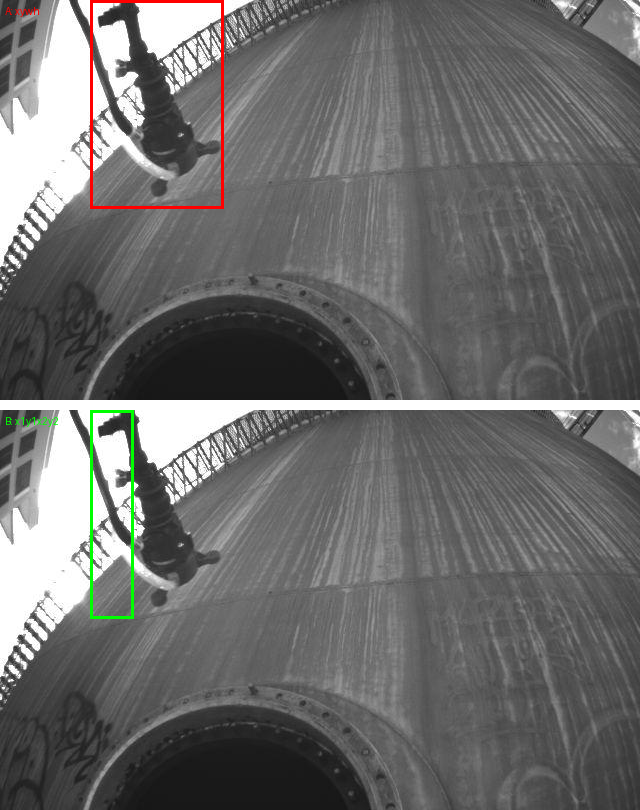
\includegraphics[width=0.55\textwidth]{figures/bbox_format_check.png}
    \caption{Comparison of the two bbox format interpretations on annotation
    \texttt{[90, 0, 133, 208]}. Top (red): \texttt{[x, y, w, h]} interpretation --- the box
    correctly encloses the probe. Bottom (green): \texttt{[x1, y1, x2, y2]} interpretation ---
    the box cuts off half of the device.}
    \label{fig:bboxcheck}
\end{figure}

\textbf{Conclusion: the format is \texttt{[x, y, w, h]}} (COCO standard), with the origin at the
top-left corner.

\subsection{Data integrity}

Automated checks performed on the dataset:

\begin{itemize}[nosep]
    \item All 308 images have size \textbf{640$\times$400 px}, with no exceptions.
    \item Images are stored as RGB JPEGs, but are in fact \textbf{grayscale} (R=G=B channels
          verified on a sample of images) --- most likely the output of a B/W or NIR camera on
          the drone.
    \item \textbf{1:1 correspondence between images and annotations}: every image has exactly
          one associated bounding box. \textbf{No ``no-probe'' examples exist} in the dataset.
    \item No bounding box falls outside the image bounds (0 out-of-bounds cases).
    \item No byte-identical duplicate images (verified via MD5 hash across all 308 images).
    \item All file names follow a fully parsable, regular pattern:\\
          \texttt{\{device\_id\}\_\{seq\}\_\{frame\}\_\{n\}flight\_\{timestamp\}\_\{cam\}.jpg}
\end{itemize}

\section{Bounding box statistics}

\subsection{Numerical summary}

\begin{table}[H]
\centering
\begin{tabular}{lrrrr}
\toprule
\textbf{Quantity} & \textbf{Min} & \textbf{Max} & \textbf{Mean} & \textbf{Median} \\
\midrule
Bbox width (px)               & 40   & 215 & 125.4 & 132.0 \\
Bbox height (px)               & 32   & 400 & 165.7 & 192.5 \\
Bbox area (\% of image)       & 0.50 & 33.6 & 8.63 & --- \\
Aspect ratio (w/h)             & 0.33 & 2.77 & 0.90 & --- \\
\bottomrule
\end{tabular}
\caption{Bounding box statistics over 308 annotations (640$\times$400 px images).}
\label{tab:bboxstats}
\end{table}

Observations:
\begin{itemize}[nosep]
    \item The object occupies on average only \textbf{8.6\% of the image area}: it is a
          small/medium target, not dominant in the frame.
    \item The maximum recorded height is \textbf{400 px}, i.e. the full image height: in cases
          where the probe's cable/arm crosses the frame vertically, the box spans the entire
          column.
    \item The aspect ratio is mostly between 0.5 and 1.3 (vertical/square shape), with a tail of
          very thin cases related to the point above.
\end{itemize}

\subsection{Probe position within the frame}

The distribution of the vertical coordinate of the bbox center (normalized, 0 = top, 1 = bottom)
is \textbf{clearly bimodal}:

\begin{itemize}[nosep]
    \item ``Top'' cluster ($c_y \in [0.05, 0.30]$): \textbf{195 images} (63\%).
    \item ``Bottom'' cluster ($c_y \in [0.65, 0.95]$): \textbf{113 images} (37\%).
\end{itemize}

This matches exactly the two variants shown in the assignment itself (``Probe attached at the
top'' / ``Probe attached at the bottom''): these are two distinct mounting/framing setups, not
noise in the data.

On the horizontal axis, the bbox center is instead skewed to the left (mean $c_x = 0.27$, range
$[0.06, 0.72]$): few cases have the probe in the right half of the image. This is relevant when
deciding whether and how much to rely on \emph{horizontal flip} during data augmentation.

\begin{figure}[H]
    \centering
    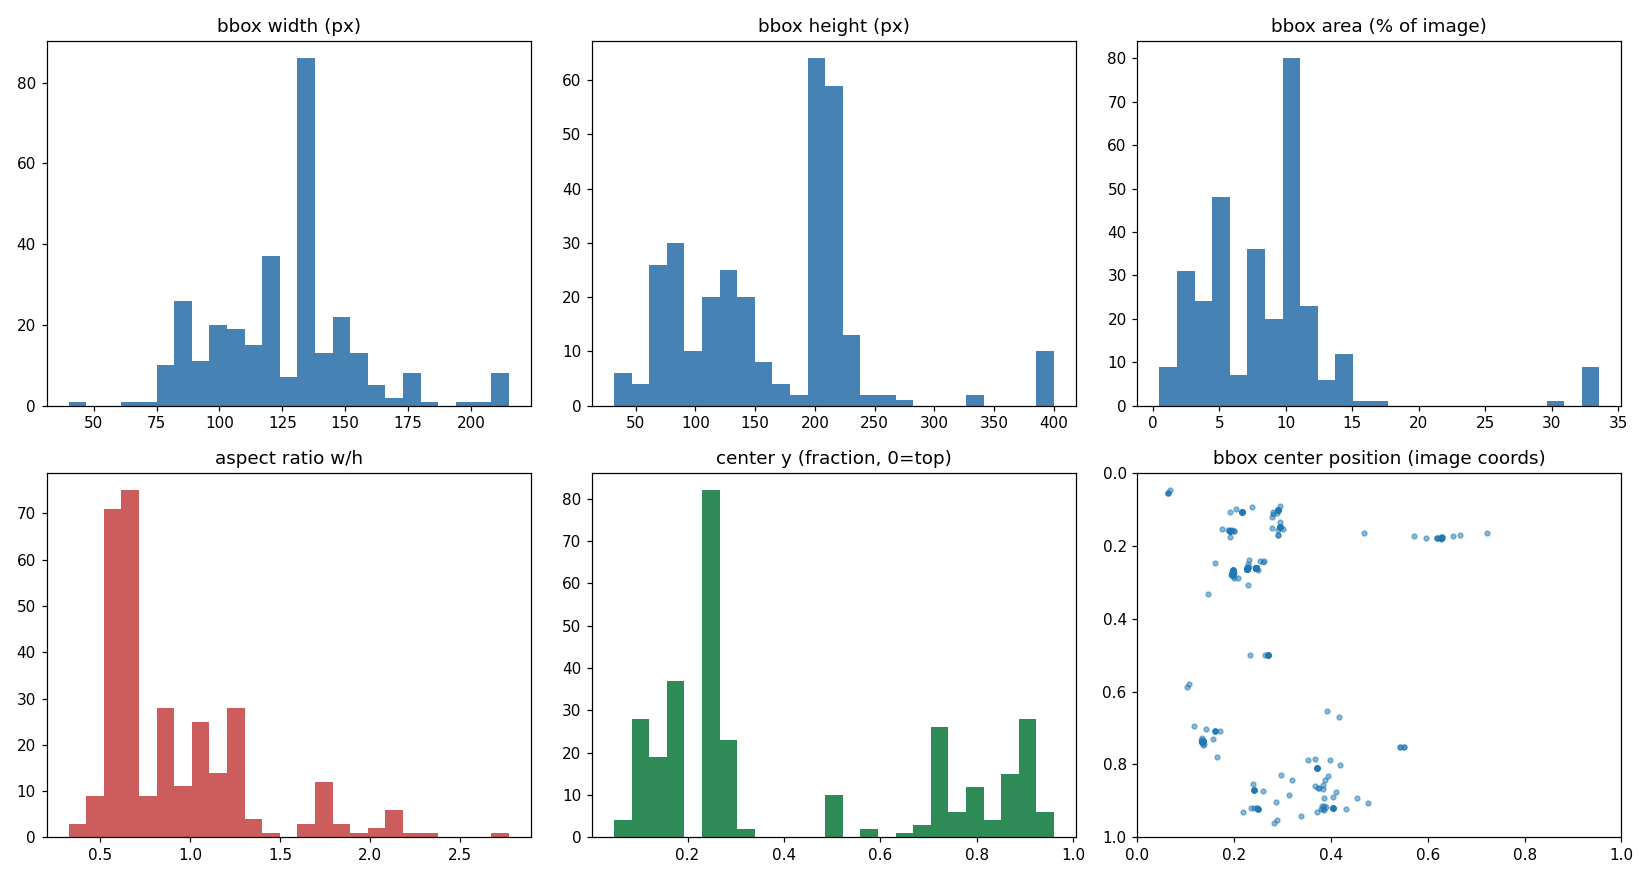
\includegraphics[width=\textwidth]{figures/dataset_stats.png}
    \caption{Statistical distributions of the bounding boxes: width, height, relative area,
    aspect ratio, vertical center position, and a scatter plot of the center position within the
    frame (image coordinates, y-axis inverted).}
    \label{fig:stats}
\end{figure}

\section{Grouping by drone and flight sequence}

Analyzing the file names reveals that the 308 images are not independent: they come from
\textbf{only 5 drones/devices} (identified by the serial number in the file name), organized
into \textbf{21 distinct flight sequences} (``flight clips''), each with a variable number of
frames ranging from 4 to 20 (average 14.7).

\begin{table}[H]
\centering
\small
\begin{tabular}{llr}
\toprule
\textbf{Device ID} & \textbf{Sequence} & \textbf{N. images} \\
\midrule
E300PREMP00002 & 00725 & 19 \\
E300PREMP00002 & 00726 & 20 \\
E300PREMP00002 & 00727 & 18 \\
E300SA22440034 & 00447 & 19 \\
E300SA22440034 & 00451 & 10 \\
E300SA22440034 & 00452 & 15 \\
E300SA22440034 & 00465 & 19 \\
E300SA22440035 & 01502 & 13 \\
E300SA22440035 & 01510 & 19 \\
E300SA22440035 & 01533 & 15 \\
E300SA23130257 & 00053 & 19 \\
E300SA23130257 & 00054 & 5 \\
E300SA23130257 & 00057 & 19 \\
E300SA23130257 & 00060 & 4 \\
E300SA23130257 & 00267 & 19 \\
E300SA23130257 & 00295 & 20 \\
E300SA23130257 & 00301 & 9 \\
EL300858804493 & 00184 & 14 \\
EL300858804493 & 00188 & 10 \\
EL300858804493 & 00193 & 4 \\
EL300858804493 & 00330 & 18 \\
\midrule
\textbf{Total} & \textbf{21 sequences} & \textbf{308} \\
\bottomrule
\end{tabular}
\caption{Number of images per (device, flight sequence).}
\label{tab:groups}
\end{table}

\textbf{Critical implication for the train/validation split}: frames belonging to the same
sequence are temporally close (same wall, same lighting, similar camera poses). A
\emph{random per-image} split would cause \textbf{data leakage} between training and validation
(near-identical frames in both splits, leading to overestimated performance). The split must be
done \textbf{per group (device, sequence)}, not per image.

A trailing tag in the file name is also noticeable (\texttt{\_0} or \texttt{\_2}, occurring 117
and 191 times respectively), most likely related to two different lenses/settings mounted on the
drone.

\subsection{Train / validation / test split}
\label{sec:groupsplit}

The implementation uses a \textbf{3-way group split} (train 70\%, val 15\%, test 15\% of
images), rather than only train/val. The reason: model-variant selection (YOLOv8 n/s/m) and
confidence-threshold calibration both use val, so val's own metrics carry some optimistic bias
from having been used to make those decisions. A test split, touched only once at the very end,
gives a more honest final number for the report.

\textbf{Limitation, stated explicitly}: with only 21 groups spread across 5 devices (two of
which have only 3 groups total each), a search over thousands of candidate group-to-split
assignments could not find one where every device is represented in every split while also
matching the target fractions and preserving the global top/bottom position ratio -- the
constraint is combinatorially too tight for this little data. The device-coverage constraint was
therefore relaxed: some devices are absent from val and/or test (present in train and at least
one other split). This means per-split metrics should not be read as equally representative of
all 5 devices, and the test-set numbers in particular carry real sampling noise given they come
from only 3--4 groups (roughly 45 images, positives and synthetic negatives combined).

\section{Qualitative observations}

\begin{figure}[H]
    \centering
    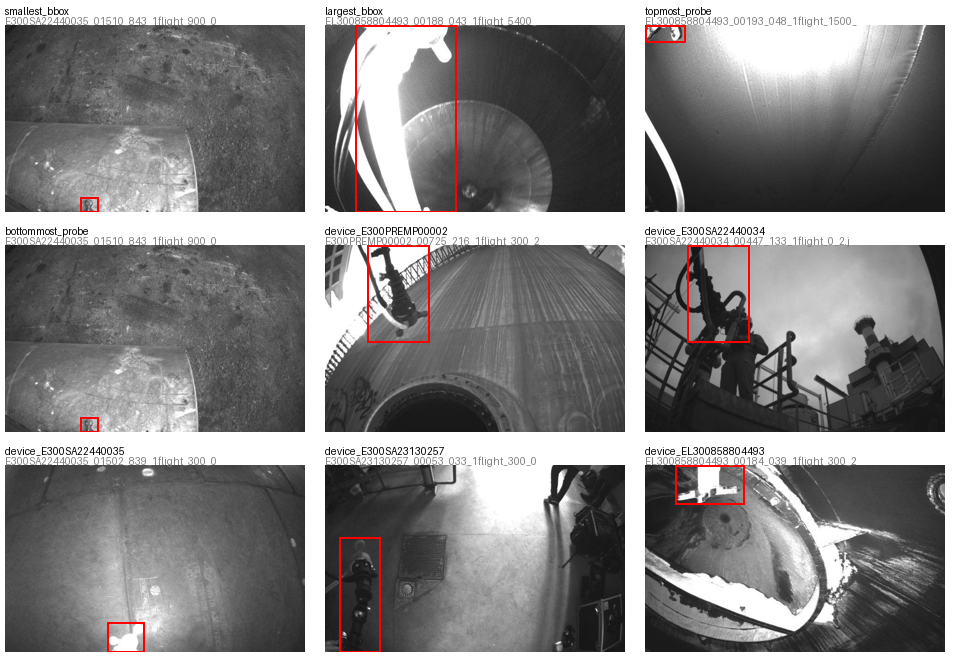
\includegraphics[width=\textwidth]{figures/sample_grid.png}
    \caption{Representative samples: smallest/largest bbox, topmost/bottommost probe position,
    and one example for each of the 5 devices present in the dataset.}
    \label{fig:samples}
\end{figure}

Visual inspection reveals a few patterns relevant to model design:

\begin{itemize}[nosep]
    \item Strong \textbf{barrel/fisheye distortion}, consistent across all images: the scenes
          show large-diameter cylindrical surfaces (most likely tanks or pipes) captured at close
          range.
    \item The background contains numerous elements that could confuse a detector: metal
          railings, rivets, structural edges, repetitive metal-surface textures.
    \item The probe is often \textbf{backlit} (overexposed sky in the background), resulting in
          low local contrast under some shooting conditions.
    \item The object is articulated (probe body + attachment arm/cable), not a rigid, compact
          blob: the bbox often also includes part of the cable.
\end{itemize}

\section{Implications for solution design}

Summary of points to keep in mind when choosing and training the model:

\begin{enumerate}[nosep]
    \item \textbf{No negative examples}: the dataset is 100\% composed of images with the probe
          present, while the final task also requires handling the ``no probe detected'' case.
          This gap needs to be addressed (e.g. via a confidence threshold on the detector,
          background crops/patches as synthetic negatives, or augmentation that removes/occludes
          the probe).
    \item \textbf{Small, low-diversity dataset}: only 21 real sequences from 5 devices. Light
          fine-tuning of a pretrained detector (e.g. YOLO, Faster R-CNN, RT-DETR) is preferable
          to training \emph{from scratch}.
    \item \textbf{Group-based split required}: the train/validation split must be based on
          (device, sequence), not on individual images, for a fair evaluation (see
          Section~\ref{tab:groups}).
    \item \textbf{Small target (8.6\% average area)}: prefer architectures/configurations with
          good sensitivity to small/medium objects (e.g. attention to higher-resolution feature
          maps, appropriate anchors/scales).
    \item \textbf{Positional bimodality and horizontal imbalance}: consider targeted augmentation
          (horizontal flip, cropping, exposure/contrast variation) rather than assuming a fixed
          probe position within the frame.
    \item \textbf{IoT deployment constraint (Jetson)}: keep this in mind already when choosing
          the architecture (e.g. models with ``nano/tiny'' variants, support for INT8
          quantization, ONNX/TensorRT export).
\end{enumerate}

\section{Model family selection}
\label{sec:modelfamily}

\subsection{Constraints driving the choice}

Two practical constraints shape which model families are realistic candidates:

\begin{itemize}[nosep]
    \item \textbf{Training hardware}: only a CPU is available locally. GPU access is possible
          through Google Colab's free tier (typically an NVIDIA T4), which is where training will
          be run; inference and final deployment remain CPU/Jetson-oriented regardless of where
          training happens.
    \item \textbf{Implementation speed and reportable depth}: given the assignment timeline, the
          chosen system must be quick to get running end-to-end, while still leaving enough of
          the pipeline under our own control to discuss and justify design choices in the report
          (this is explicitly part of the evaluation criteria).
\end{itemize}

\subsection{Macro comparison by model family}

\begin{table}[H]
\centering
\small
\begin{tabular}{p{2.6cm}p{3.2cm}p{3.2cm}p{3.4cm}}
\toprule
\textbf{Family} & \textbf{Training cost (CPU / Colab GPU)} & \textbf{Implementation speed} & \textbf{Depth demonstrable in report} \\
\midrule
One-stage CNN (YOLO family: v8/11/v12/26) &
Low --- light fine-tuning from COCO-pretrained weights converges in a handful of epochs even on
a single free GPU, and is still tractable on CPU for a dataset this small &
Very high --- mature, well-documented framework (Ultralytics), training/eval/export in a few
lines &
Medium --- most of the pipeline is handled by the framework, less custom code to discuss \\
\addlinespace
Two-stage / anchor-based CNN (Faster R-CNN, RetinaNet) &
Moderate --- heavier per-step compute than YOLO, but still feasible with light fine-tuning
(frozen backbone + few epochs) on a Colab GPU &
Medium --- pretrained weights available in torchvision, but the training loop, augmentation and
COCO-style evaluation are largely hand-written &
High --- full visibility and control over RPN/anchors/losses, better material for a
deep-learning-focused report \\
\addlinespace
Transformer-based (RT-DETR, RF-DETR, D-FINE) &
High --- transformers typically need more iterations/data to converge reliably; risky within a
308-image, 21-sequence dataset and a limited Colab session budget &
Low to medium --- RT-DETR has reasonably mature tooling, but RF-DETR/D-FINE are young
repositories with less documentation and a higher chance of integration friction &
High in principle (attention, set prediction, no NMS), but the risk of spending time on plumbing
instead of results is significant \\
\bottomrule
\end{tabular}
\caption{Macro-level comparison of object detection model families against the constraints
described in Section~\ref{sec:modelfamily}.}
\label{tab:modelfamily}
\end{table}

\subsection{Decision}

The transformer-based family is deprioritized: the combination of a small, low-diversity
dataset and CPU/limited-GPU training budget makes it the riskiest option for the
lowest expected benefit within this assignment's scope.

The shortlist is narrowed to the two CNN-based families:
\begin{itemize}[nosep]
    \item \textbf{YOLO family (Ultralytics)} --- pragmatic choice, fastest to implement,
          strong built-in augmentation, mature export path to ONNX/TensorRT for the Jetson
          deployment question raised in the assignment.
    \item \textbf{Faster R-CNN / RetinaNet (torchvision)} --- more implementation effort, but
          more material to demonstrate understanding of the underlying mechanics (anchors, RPN,
          losses) in the report.
\end{itemize}

\textbf{Update}: following further discussion, the scope was narrowed to \textbf{YOLOv8 only}
(no Faster R-CNN/RetinaNet comparison baseline), to keep implementation effort focused given the
timeline. The specific variant (n/s/m) is decided empirically in
Section~\ref{sec:nextsteps}'s training step, by comparing them directly on this dataset's val
split rather than committing to one upfront.

\subsection{Training environment: Google Colab + Google Drive}

Training will run on Google Colab rather than locally, to remove the CPU bottleneck. Practical
workflow notes:

\begin{itemize}[nosep]
    \item Dataset (\texttt{probe\_images/} + \texttt{probe\_labels.json}) is uploaded to Google
          Drive and the Drive is mounted in the Colab notebook.
    \item At the start of each session, the dataset is copied from the mounted Drive into the
          Colab VM's local disk (\texttt{/content/...}) before training: reading thousands of
          small JPEG files directly over the mounted Drive is slow, whereas local VM disk I/O is
          fast. The local copy is not persistent across sessions, so this copy step is repeated
          each time.
    \item Checkpoints/weights are saved back to Drive periodically during training (not only to
          the local VM disk), since free Colab sessions can disconnect on idle timeout or after
          reaching the session length limit ($\sim$12h), which would otherwise lose anything not
          written to persistent storage.
    \item Inference (\texttt{inference.py}) and final deployment remain independent of this
          training environment and are designed to run on CPU / Jetson.
\end{itemize}

\section{Handling the absence of negative examples}
\label{sec:negatives}

\subsection{Why this matters}

Every one of the 308 training images contains exactly one probe (Section~2.2). This is a real
gap with respect to the final task, which explicitly requires the system to report when no probe
is detected.

It is worth being precise about what is and is not already covered by the current data:
\begin{itemize}[nosep]
    \item Standard object detection training already treats most of the area within each image
          as background/negative at the region or anchor level (the probe covers only 8.6\% of
          the image on average, Section~3), so the model does receive plenty of implicit negative
          supervision during training.
    \item What is genuinely missing is \textbf{full images that contain no probe at all}: the
          model has never seen a complete scene without the object, and --- more importantly ---
          there is currently no way to calibrate or evaluate the ``no probe detected'' behavior,
          since doing so requires true negative examples in the validation set (to measure
          false-positive rate and tune the confidence threshold).
\end{itemize}

\subsection{Strategy: synthetic negatives via generative inpainting}

\begin{enumerate}[nosep]
    \item \textbf{Confidence thresholding (baseline, already available)}: report ``no probe
          detected'' whenever no detection exceeds a chosen confidence threshold. Free, but the
          threshold needs real negative signal to be calibrated rather than guessed.
    \item \textbf{Synthetic true negatives (implemented)}: using the known bbox for each image,
          mask out the (padded) probe region and fill it in, producing a ``probe-absent''
          counterpart of the same scene. This generates one realistic full-negative image per
          original, spanning every device, flight sequence and lighting condition already
          present, at near-zero additional labeling cost.
    \item \textbf{Real negative frames (future work, not pursued)}: only 4--20 frames per flight
          sequence were selected for labeling out of what is presumably a much longer raw flight
          (Section~4). If the raw footage were available, pulling and manually verifying
          probe-free frames directly from the source would give the most reliable negatives, but
          this was outside this assignment's scope/time budget.
\end{enumerate}

\textbf{Fill method: classical inpainting was tried first and rejected.} \texttt{cv2.inpaint}
(Telea / Navier-Stokes texture propagation, not a learned model) was tested first, since it
requires no extra dependencies. Visual QA (a before/after contact sheet over a sample biased
towards the largest bboxes) showed it looks convincing for small/medium bboxes ($\lesssim$20\%
of image area), but produces a visibly blurred band for the largest ones (up to $\sim$33\% of
image area, concentrated in one flight sequence) -- a real risk, since the model could learn to
associate that blur artifact, rather than genuine scene understanding, with ``no probe''. A
background-crop fallback (reusing a real, non-overlapping region of the same image, resized back
to full frame) was implemented as a first mitigation, but introduces a second, subtler
inconsistency: two visibly different negative ``styles'' correlated with the source bbox size,
itself a potential shortcut.

The negatives actually shipped in \texttt{yolo\_dataset/} use \textbf{LaMa} (Large Mask
Inpainting), a model trained specifically to hallucinate plausible content for large masked
regions, applied uniformly regardless of bbox size. Re-running the same QA process with LaMa
confirmed convincing results across the full bbox-size range, including the previously
problematic large-bbox sequence -- see \texttt{data\_prep/negatives\_qa/contact\_sheet.png}. LaMa
is not part of the main training/inference environment (it pulls in older numpy/opencv/pillow
versions than the rest of the stack); it runs in a separate \texttt{.venv-lama} environment used
only to (re)build the dataset offline, keeping the main environment's dependencies clean and
reproducible.

\textbf{Key point}: negative examples matter as much for \textbf{evaluation} as for training. The
val and test splits each include a slice of synthetic negative images so that the false-positive
rate and the confidence threshold itself can be measured and tuned, rather than assumed.

\subsection{Quality-review heuristic}

A lightweight heuristic score (\texttt{score\_negative\_quality} in
\texttt{data\_prep/generate\_negatives.py}) flags which generated negatives are worth a manual
look: the ratio of the filled region's sharpness to that of a real surrounding ring in the same
image (block-median Laplacian variance, robust to a small unrelated high-contrast region --
e.g. a real building edge -- skewing a plain average). Two rounds of correction were needed
after checking specific low-scoring cases against the actual images: an early version compared
against a context patch that still included the filled region itself, inflating scores; the
corrected, ring-based version is more honest but pushes scores down across the board, since
generated fills are inherently a bit smoother than real sensor grain even when they look
convincing. \textbf{No absolute pass/fail cutoff is used} -- verified false positives include a
fill next to a real, naturally low-texture sky/building boundary, and a fill over a saturated,
naturally textureless light reflection. The score is used only as a relative ranking (lowest
first) to prioritize manual review, never to auto-exclude images.

\subsection{Negative ratio: per-split, not uniform}

The train split uses a lower negative ratio than val/test (\texttt{--train-neg-ratio 0.3} vs.
\texttt{1.0} for val/test, in \texttt{data\_prep/build\_yolo\_dataset.py}). Reasoning: a
negative image contributes no localization learning signal at all (there is no GT box to
regress against, only a classification/objectness signal), so a 1:1 ratio in \emph{training}
mostly dilutes how often the model sees real positive examples per epoch without a clear
benefit. val/test negatives, by contrast, are exactly what calibrates the confidence threshold
and measures the false-positive rate -- shrinking those would make that measurement noisier, so
they keep full negative coverage. Negatives are pruned from the already-generated files rather
than regenerated at a lower ratio (\texttt{data\_prep/select\_negatives.py}), since the fill
images on disk don't need to change, only which ones are included.

\section{Implementation status}
\label{sec:nextsteps}

\begin{itemize}[nosep]
    \item[\checkmark] Train/val/test split by flight group (Section~\ref{sec:groupsplit}),
          synthetic negatives via LaMa, COCO-to-YOLO dataset build
          (\texttt{data\_prep/build\_yolo\_dataset.py}).
    \item[\checkmark] \texttt{inference.py} implemented and smoke-tested end-to-end with a stock
          pretrained checkpoint (mechanics only -- meaningful detections require the fine-tuned
          weights from the step below).
    \item[\checkmark] \texttt{evaluate.py} implemented: localization (mean IoU, Precision/
          Recall/F1/AP@0.5), no-probe false-positive rate and threshold calibration, CPU runtime
          -- selectable per split (\texttt{--split val/test}) so val can be used for
          development decisions and test only once, at the end.
    \item[\checkmark] \texttt{compare\_results.py}: bar-chart comparison across multiple
          \texttt{evaluate.py} runs, used both to quantify the out-of-the-box pretrained baseline
          vs. the fine-tuned model, and to compare the YOLOv8 n/s/m variants against each other.
    \item[ ] \textbf{Remaining}: run the actual fine-tuning on Google Colab
          (\texttt{training/train\_colab.ipynb}) across the n/s/m variants, pick the final model
          empirically, run the one-time test-split evaluation, and fold the resulting numbers
          and figures into the final report.
\end{itemize}

\end{document}
